\documentclass[a4paper,11pt]{jsarticle}


% 数式
\usepackage{amsmath,amsfonts,amssymb}
\usepackage{bm}
% 画像
\usepackage[dvipdfmx]{graphicx}
\usepackage[dvipdfmx]{color}
\usepackage{siunitx}
\usepackage{wrapfig}
\usepackage{cases}
\usepackage{dcolumn}
\makeatletter
\newcommand{\figsubcaption}[1]{\def\@captype{figure}\subcaption{#1}}
\newcommand{\tblsubcaption}[1]{\def\@captype{table}\subcaption{#1}}
\makeatother

% サブキャプション
\usepackage{subcaption}

\usepackage{listings,jvlisting}
\lstset{
basicstyle={\ttfamily},
identifierstyle={\small},
commentstyle={\smallitshape},
keywordstyle={\small\bfseries},
ndkeywordstyle={\small},
stringstyle={\small\ttfamily},
frame={tb},
breaklines=true,
columns=[l]{fullflexible},
numbers=left,
xrightmargin=0zw,
xleftmargin=3zw,
numberstyle={\scriptsize},
stepnumber=1,
numbersep=1zw,
lineskip=-0.5ex
}

\begin{document}

\title{2重振り子を長さと慣性モーメントが時間変化する単振り子としてみる}
\author{平林広}
\date{\today}
\maketitle


\begin{figure}[h]
  \centering
  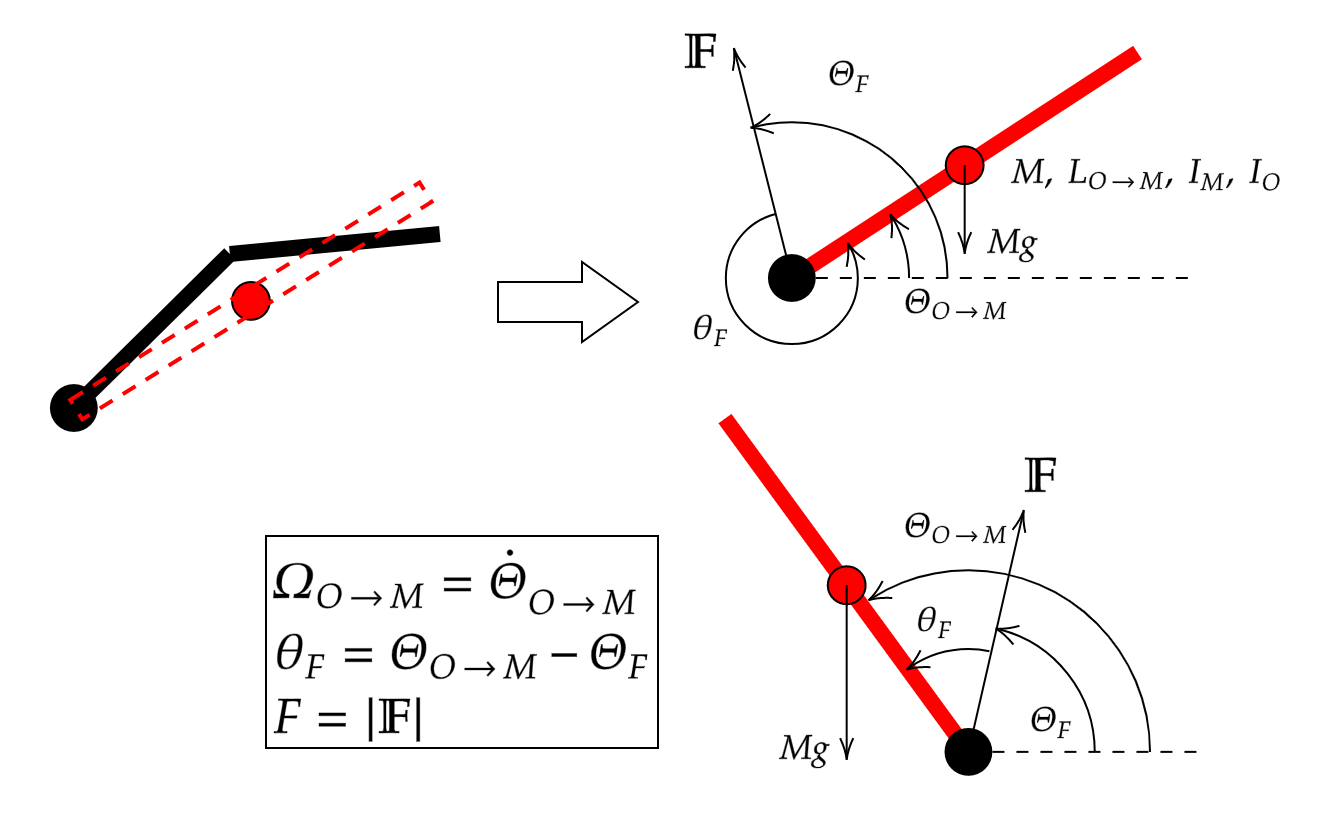
\includegraphics[width = 0.8\textwidth]{config.png}
  \caption{変数設定}
  \label{config.png}
\end{figure}

\begin{figure}[h]
  \centering
  \begin{tabular}{ccccc}
    \begin{minipage}[t]{0.15\textwidth}
      \centering
      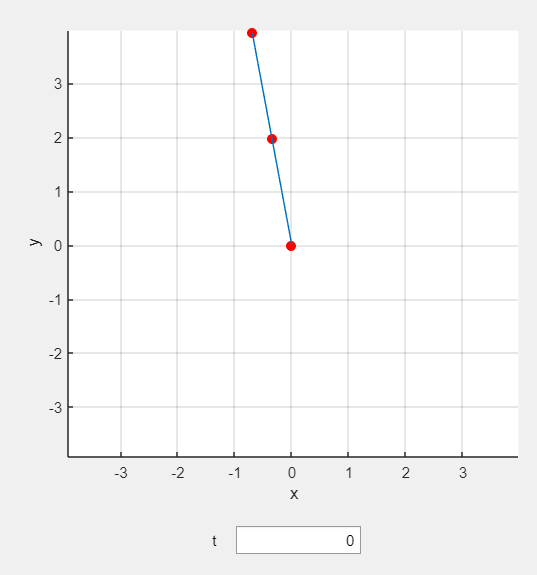
\includegraphics[width=1\textwidth]{2seg_movement_01.png}
      \subcaption{$t=0$}
    \end{minipage} &
    \begin{minipage}[t]{0.15\textwidth}
      \centering
      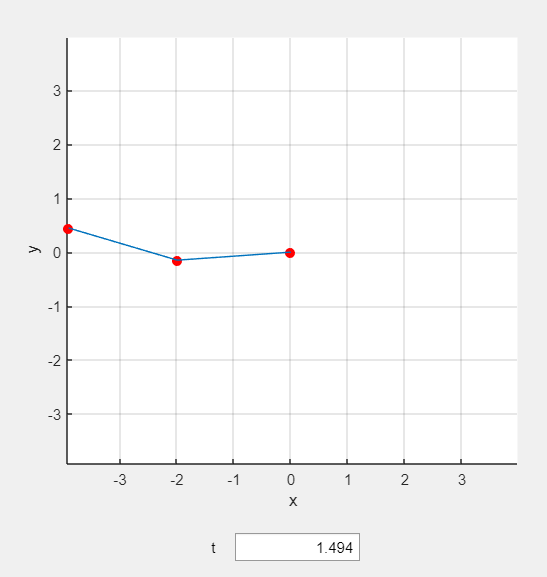
\includegraphics[width=1\textwidth]{2seg_movement_02.png}
      \subcaption{$t=1.494$}
    \end{minipage} &
    \begin{minipage}[t]{0.15\textwidth}
      \centering
      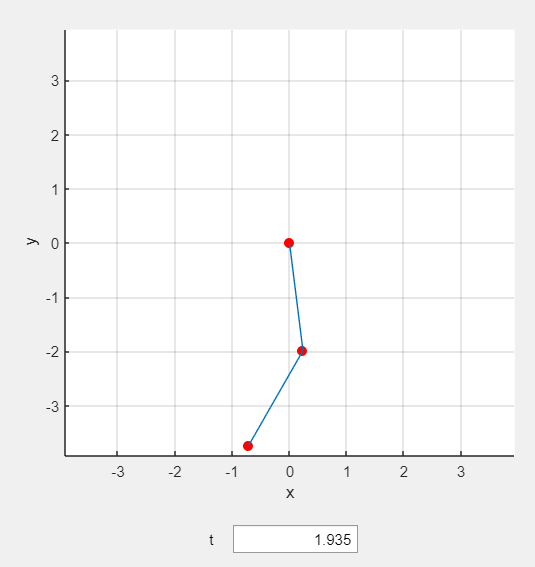
\includegraphics[width=1\textwidth]{2seg_movement_03.png}
      \subcaption{$t=1.907$}
    \end{minipage} &
    \begin{minipage}[t]{0.15\textwidth}
      \centering
      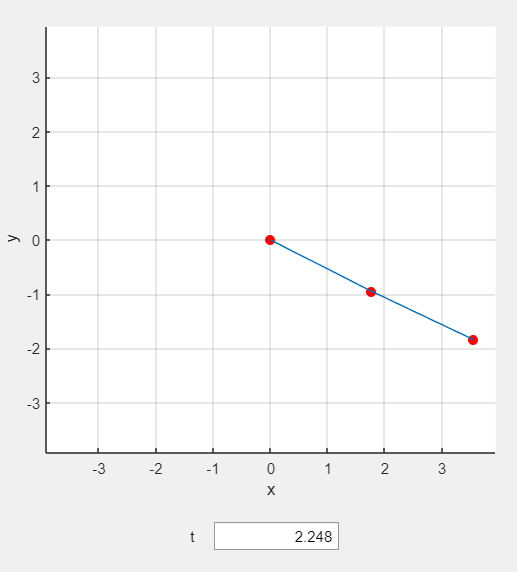
\includegraphics[width=1\textwidth]{2seg_movement_04.png}
      \subcaption{$t=2.134$}
    \end{minipage} &
    \begin{minipage}[t]{0.15\textwidth}
      \centering
      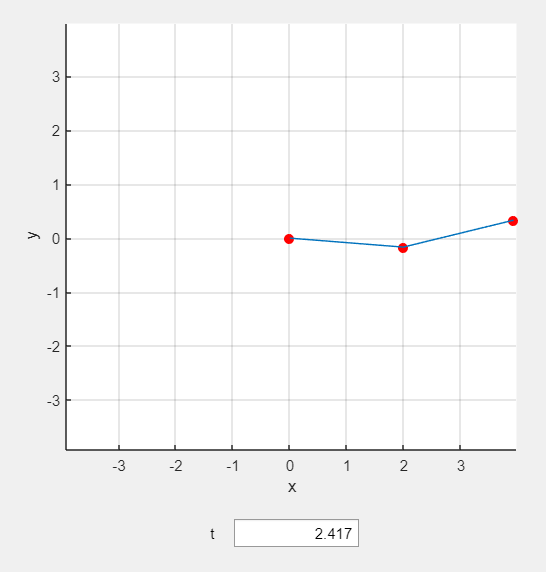
\includegraphics[width=1\textwidth]{2seg_movement_05.png}
      \subcaption{$t=2.417$}
    \end{minipage}
  \end{tabular}
  \caption{
    適用した2重振り子の様子。
    1セグメント目が真下になるまで
    2セグメント目が負に一定の加速度を持つようなトルクを発生させ、
    1セグメント目が真下以降は
    2セグメント目が正に一定の加速度を持つようなトルクを発生させた。
  }
  \label{2seg_example}
\end{figure}

ニュートンの運動方程式は
動径方向(内向きを正)、
固定点周りの角運動量変化$\left(\frac{d}{dt}\left(I_O\Omega_{O\rightarrow M}\right)\right)$、
重心周りの角運動量変化$\left(\frac{d}{dt}\left(I_M\Omega_{O\rightarrow M}\right)\right)$について成り立つ。
\begin{gather*}
  \begin{cases}
    ML_{O\rightarrow M}{\Omega_{O\rightarrow M}}^2 - M\ddot{L}_{O\rightarrow M} = Mg\sin\Theta_{O\rightarrow M} - F\cos\theta_F
    \\
    \dot{I}_O \Omega_{O\rightarrow M} + I_O \dot{\Omega}_{O\rightarrow M} = -Mg\cos\Theta_{O\rightarrow M} L_{O\rightarrow M}
    \\
    \dot{I}_M \Omega_M + I_M \dot{\Omega}_{O\rightarrow M} = F\sin\theta_F L_{O\rightarrow M}
  \end{cases}
\end{gather*}

図\ref{2seg_example}のような2重振り子に適用して、両辺を計算してみる.
すると
動径方向に関する方程式は成り立つことが分かるが、
固定点周りの角運動量変化$\left(\frac{d}{dt}\left(I_O\Omega_{O\rightarrow M}\right)\right)$と
重心周りの角運動量変化$\left(\frac{d}{dt}\left(I_M\Omega_{O\rightarrow M}\right)\right)$
に関しては成り立たないことが分かる。
途中までは一致しているように見えるが、それはセグメント間のトルクが小さいためそう見えるだけである。
数値的に重心周りの角運動量を計算し、その微分をとると、それは右辺と一致することが分かる。
\begin{figure}[h]
  \centering
  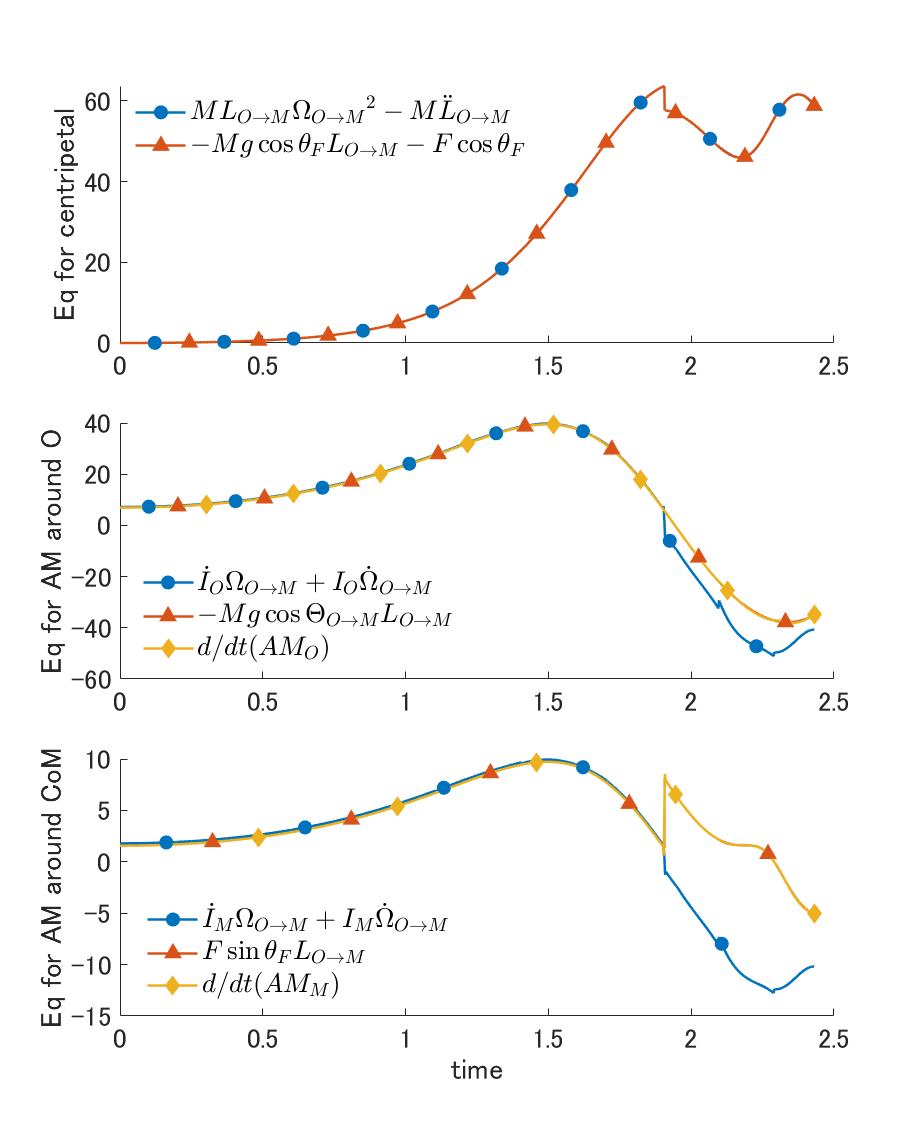
\includegraphics[width = 0.75\textwidth]{equation_values.png}
  \caption{
    各方程式の左辺と右辺の値。
    $AM$は2重振り子としての全体の重心周りの角運動量。
  }
  \label{equation_values.png}
\end{figure}

これは
固定点周りの角運動量$I_O\Omega_{O\rightarrow M})$と
重心周りの角運動量$I_M\Omega_{O\rightarrow M}$が
正しくないからである
(図 \ref{AM_compare.png})。

\begin{figure}[b]
  \centering
  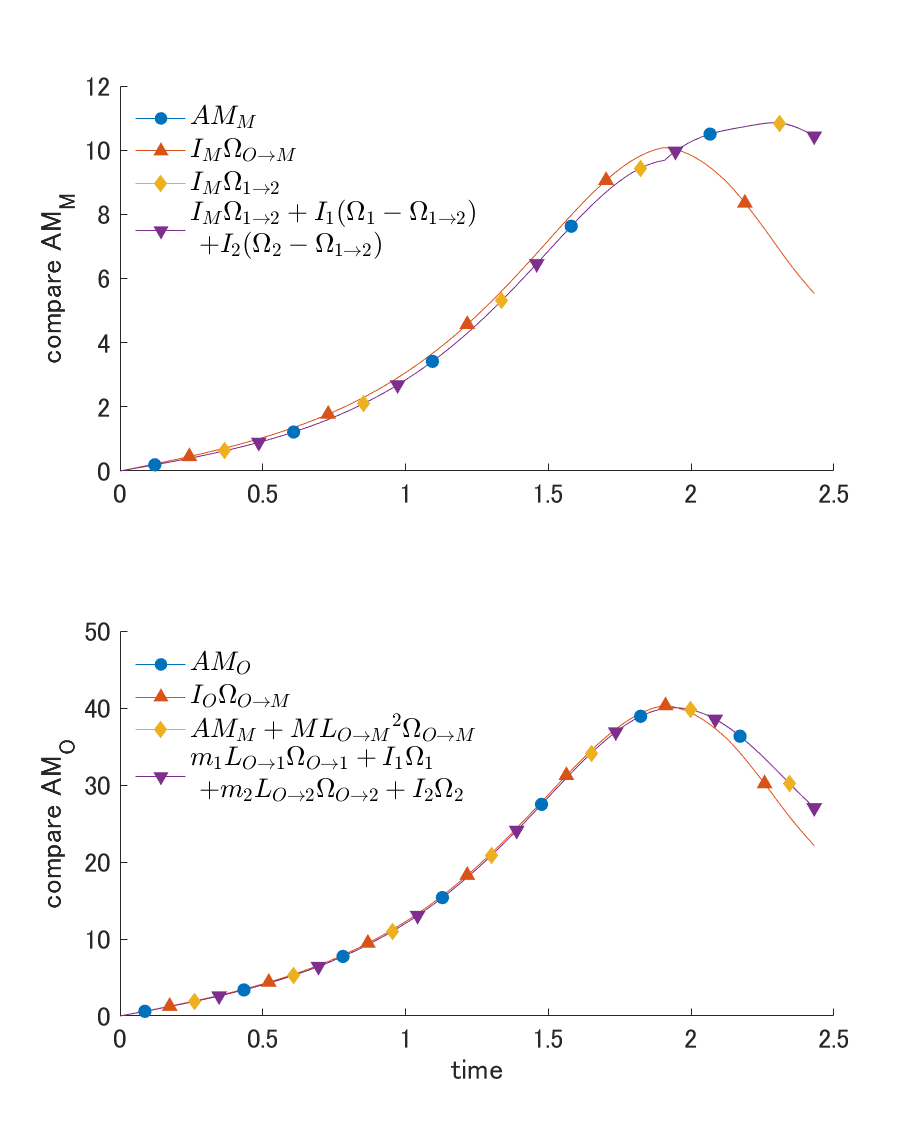
\includegraphics[width = 0.75\textwidth]{AM_compare.png}
  \caption{様々な計算でだす角運動量もどき}
  \label{AM_compare.png}
\end{figure}

重心周りの角運動量が正しくないのは、
重心周りに各セグメントの重心がどれだけ回転しているかを正しく計算できていないからである。
固定点と重心を結ぶ線分上に各セグメントの重心はなく、
それゆえ固定点と重心を結ぶ線分の回転から角運動量は計算できない。
各セグメントの重心を結ぶ線分の角速度で大体近似できるが、
それは各セグメントの重心の動きによって発生する角運動量に対して、
各セグメントが回転することで発生する角運動量
$\left[I_1(\Omega_1-\Omega_{O\rightarrow M})+I_2(\Omega_1-\Omega_{O\rightarrow M})\right]$
が十分に小さいからである。

固定点周りも同様に一致しない様子が見られる。
これも同様に角速度が正しく計算できていないからである。
平行軸の定理が成り立つことは確認できる。
ちなみに、しっかりと固定点周りの角運動量を計算すると
$\Omega_{1\rightarrow 2}$は登場しない。
固定点とセグメント1を結んだ線分の角速度、
固定点とセグメント2を結んだ線分の角速度は
セグメント1とセグメント2を結んだ線分の角速度と関係がないからである。

\end{document}